\subsection{JARVIS-Leaderboard}
{{\footnotesize
\noindent JARVIS-Leaderboard is a community-driven platform benchmarking AI, electronic
structure, force-fields, quantum computing, and experimental methods across hundreds
of materials science tasks.


\begin{description}[labelwidth=4cm, labelsep=1em, leftmargin=4cm, itemsep=0.1em, parsep=0em]
  \item[date:] 2023-06-20
  \item[version:] 1
  \item[last\_updated:] 2023-06-20
  \item[expired:] false
  \item[valid:] yes
  \item[valid\_date:] 2023-06-20
  \item[url:] \href{https://arxiv.org/abs/2306.11688}{https://arxiv.org/abs/2306.11688}
  \item[doi:] 10.48550/arXiv.2306.11688
  \item[domain:] Materials Science; Benchmarking
  \item[focus:] Comparative evaluation of materials design methods
  \item[keywords:]
    - leaderboards
    - materials methods
    - simulation
  \item[licensing:] NIST
  \item[task\_types:]
    - Method benchmarking
    - Leaderboard ranking
  \item[ai\_capability\_measured:]
    - Performance comparison across diverse materials design methods
  \item[metrics:]
    - MAE
    - RMSE
    - Accuracy
  \item[models:]
    - unkown
  \item[ml\_motif:]
    - Material science
  \item[type:] Benchmark
  \item[ml\_task:]
    - Supervised Learning
  \item[solutions:] 0
  \item[notes:] 1281 contributions across 274 benchmarks
  \item[contact.name:] Kamal Choudhary
  \item[contact.email:] kamal.choudhary@nist.gov
  \item[datasets.links.name:] AI model specific benchmarks
  \item[datasets.links.url:] \href{https://pages.nist.gov/jarvis\_leaderboard/AI/}{https://pages.nist.gov/jarvis\_leaderboard/AI/}
  \item[results.links.name:] unknown
  \item[results.links.url:] \href{unknown}{unknown}
  \item[fair.reproducible:] True
  \item[fair.benchmark\_ready:] True
  \item[id:] jarvis-leaderboard
  \item[Citations:] \cite{choudhary2024jarvis}
\end{description}

{\bf Ratings:} ~ \\

\begin{tabular}{p{0.15\textwidth} p{0.07\textwidth} p{0.7\textwidth}}
\hline
Rating & Value & Reason \\
\hline
dataset & 4 & Data is public and adheres to FAIR principles across the NIST-hosted infrastructure; however, metadata completeness varies slightly across benchmarks. No splits.
 \\
documentation & 1 & Only the task is specified.
 \\
metrics & 5 & Metrics stated for each benchmark.
 \\
reference\_solution & 4 & Many baselines across tasks (CGCNN, ALIGNN, M3GNet, etc.); no constraints specified.
 \\
software & 1 & Setup script provided, but no code provided
 \\
specification & 1 & Only dataset format is defined.
 \\
\hline
\end{tabular}

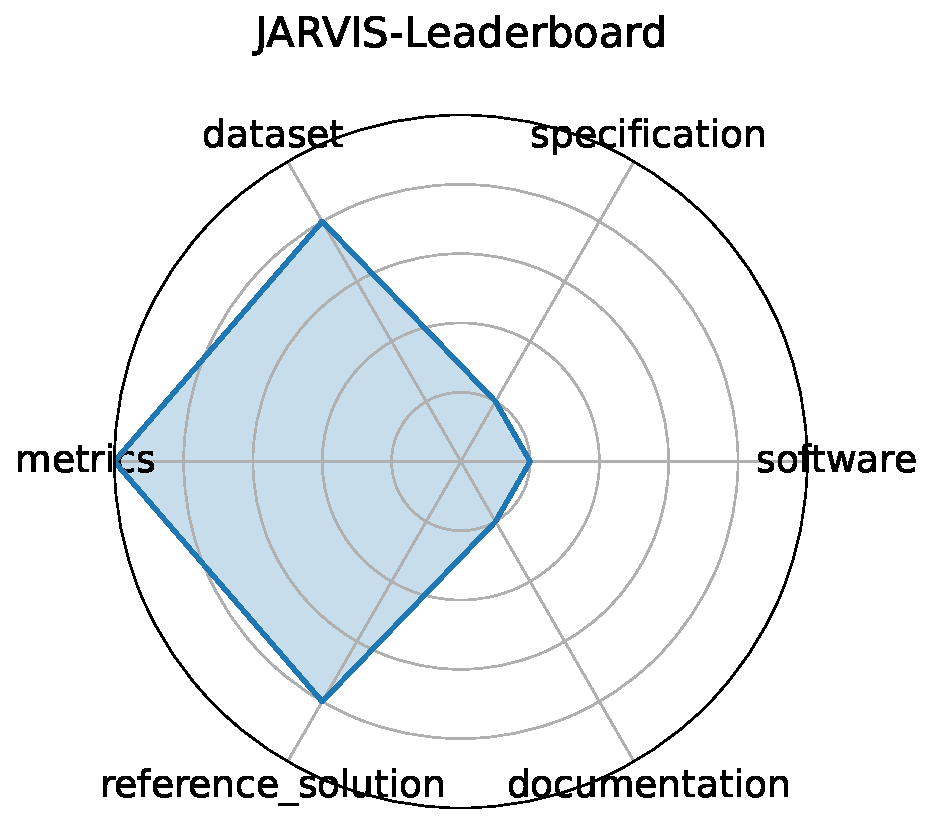
\includegraphics[width=0.2\textwidth]{jarvis-leaderboard_radar.pdf}
}}
\clearpage